\chapter{Introduction}

\section{Context of the internship}

As part of my 4 year of engineering degree at Polytech Grenoble in computer science, I completed my 12-week internship at Universiti Teknologi PETRONAS (UTP) in Seri Iskandar, Malaysia. This internship took place from \textbf{May 20, 2019} to \textbf{August 9, 2013}.

On the occasion of the establishment of a future partnership between Polytech Grenoble and UTP, various internship topics were sent to us by the Polytech International Relations Office. In the end, four of us decided to go to UTP: I was accompanied by two other students from the INFO speciality (Computer Science) and a student from IESE (Computer Science and Electronics of Embedded Systems).


\begin{figure}[h]
  \centering
  \begin{subfigure}{.5\textwidth}
    \centering
    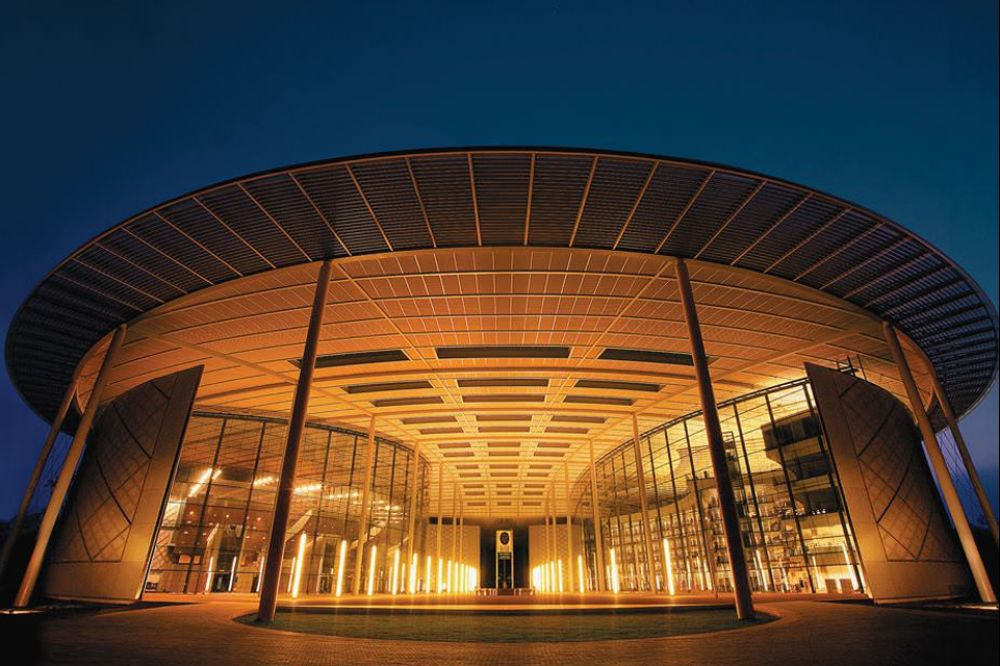
\includegraphics[width=.8\linewidth]{content/imgs/utp.jpg}
    \caption{University library}
  \end{subfigure}%
  \begin{subfigure}{.5\textwidth}
    \centering
    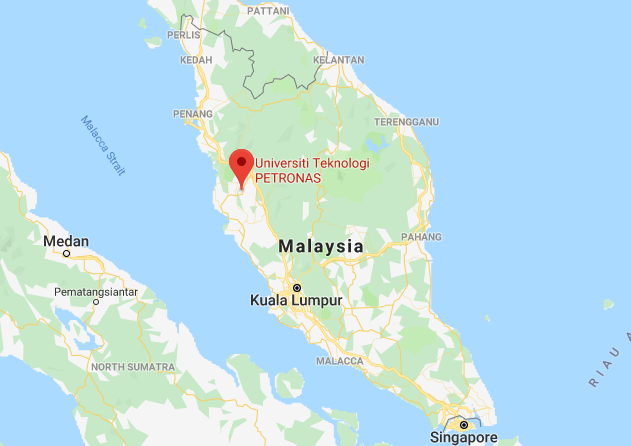
\includegraphics[width=.8\linewidth]{content/imgs/map.png}
    \caption{UTP, Seri Iskandar, Malaisie}
  \end{subfigure}
  \caption{Universiti Teknologi PETRONAS}
\end{figure}




\section{Proposed topic}

The subject that has been proposed to me aims to develop a mobile application  to help people with stuttering to heal.

According to \textit{Wikipedia}\cite{def_wiki}, stuttering is a speech disorder affecting the flow of speech characterized by involuntary repetitions and extensions of sounds, syllables, words or sentences, and involuntary silent pauses in which the "stutter" (term referring to an individual with a stuttering or related disorder) is unable to produce a sound.

A similar application has already been developed over three years by students as part of their final year project. As illustrated in appendix \ref{appendix:old_app}, this application offers the following features:

\begin{itemize}
  \item Exercises to learn how to control the speech flow;
  \item The possibility to visualize progress for each exercise (in list form, and for some exercises in graphical form);
  \item Information about stuttering.
\end{itemize}

This application was available on Android devices via the Play Store, the application store developed by Google Inc. Due to too many bugs returns about the application, it had to be removed from the Play Store.

The subject that has been proposed to me is to start again from the beginning the development of this application, taking again the functionalities previously presented.

In its final version, the application will therefore have to offer different exercises to learn how to control its speech flow as well as the possibility to visualize its progress for each of the exercises (with graphs illustrating the user's progress). In addition, the application can be used by speech therapists to access their patients' progress. They will be able to leave a comment on the exercises carried out by their participants to help them progress.

No other constraints (technology to be used, work organization, etc.) were imposed.


\section{Purpose of the report}
This report is intended for anyone who wants to have an overview of the project and what has been achieved during the 12 weeks of the project. In particular, this report is a good entry point for all those who wish to continue the development of \textit{Stuttherapy}. The report is available in English and French.

\section{Organization of the report}

The report is first of all made up of this part, the introduction. I first presented the context in which the internship was carried out and then gave a brief description of the proposed topic.

Then, the second part describes the work actually done during this internship, including the whole process of reflection, research, design, organization, development and testing.

Before concluding this report, a page will be devoted to sustainable development, in accordance with the 2009 Grenelle 1 law on the environment.

Finally, the report will review the knowledge I have acquired and improved over the past 12 weeks. 























%
